\begin{problem}{填色}{standard input}{standard output}{1 second}{128 megabytes}

    欢迎来到\textit{北京理工大学第十四届“连山科技”程序设计大赛}。命题人秉承着 “让题目在题面友好的基础上有一点点思维难度” 的出题原则,为大家安排了一些好玩又有趣的算法题。
    
    为了向大家展示命题人的友好,咱们接着来复习一下数学知识吧:

    \begin{center}
        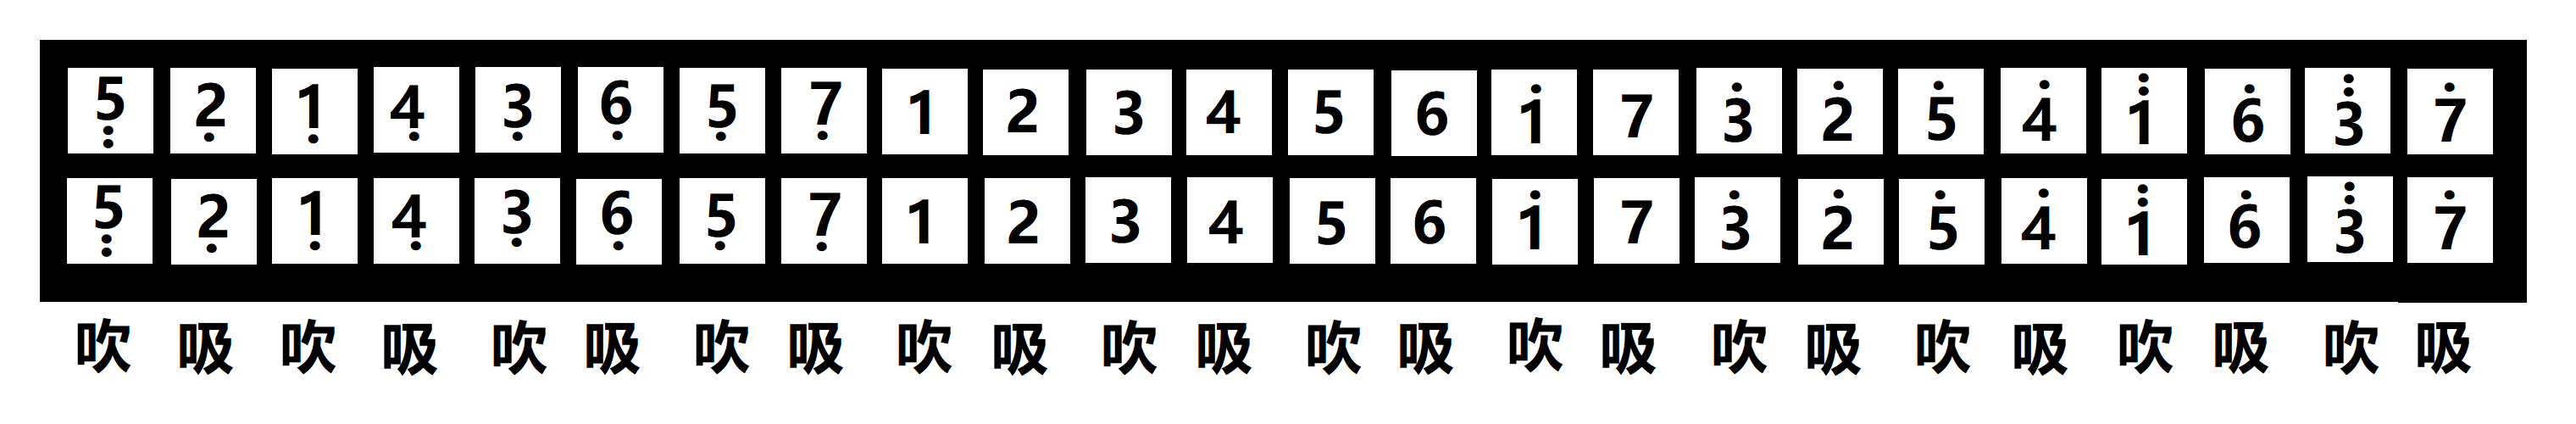
\includegraphics[width=6cm]{1.png}
    \end{center}

    如上图,在 $1\times n$ 的网格图中,每个网格都可以被蜡笔涂上一种颜色,但是要求相邻网格的颜色不能相同。现在提供 $n$ 种颜色的蜡笔以及一张部分网格已经被龙龙涂上了某些颜色的绘画图。请聪明的你算一算,在满足相邻网格的颜色不能相同的条件下把整幅网格图都涂满颜色的方案数是多少呢?


    \InputFile
    
    第一行输入一个正整数 $T\ (1\le T\le 10)$,表示数据组数。
    
    接下来 $T$ 组数据,每组数据第一行输入三个正整数 $n\ (1\le n\le 100)$、$a$ 和 $b\ (1\le a,b\le n)$,描述这幅图为 $1\times n$ 的网格,其中第一个网格被涂上了颜色 $a$,最后一个网格被涂上了颜色 $b$,其它的网格都尚未着色。
    
    \OutputFile
    
    请输出一个非负整数,表示在满足相邻网格的颜色不能相同的条件下把整幅网格图都涂满颜色的方案数,答案可能很大,请取模 $20190413$。
    
    \Example
    
    \begin{example}
    \exmp{
        2
        3 1 2
        4 2 2
    }{
        1
        6
    }%
    \end{example}

    \Explanation

    对于样例一,填法只有\texttt{[312]}这一种。
    
    对于样例二,填法有\texttt{[2132]}、\texttt{[2142]}、\texttt{[2312]}、\texttt{[2342]}、\texttt{[2412]}和\texttt{[2432]}总计 $6$ 种。

\end{problem}